
\section{Plotting Functions}
\label{sec:plotting}

The fringe fitting procedure in HOPS3 is tightly coupled with plotting, which is handled through PGPLOT. PGPLOT has been unsupported for many years and it will not be a required dependency in \nuHOPS. In \nuHOPS, fringe-fitting and plotting will be decoupled (fringe results can be generated and saved, with or without generating a plot), and the native plotting functions will be replaced with new code. We have prototyped a set of Matplotlib functions that reproduce the standard ``fringe'' plot generated by fourfit (see Figure~\ref{fig:matplotlib-fringe-plot}).

\begin{figure}[h!]
  \begin{center}
    \captionsetup{width=0.6\linewidth}
    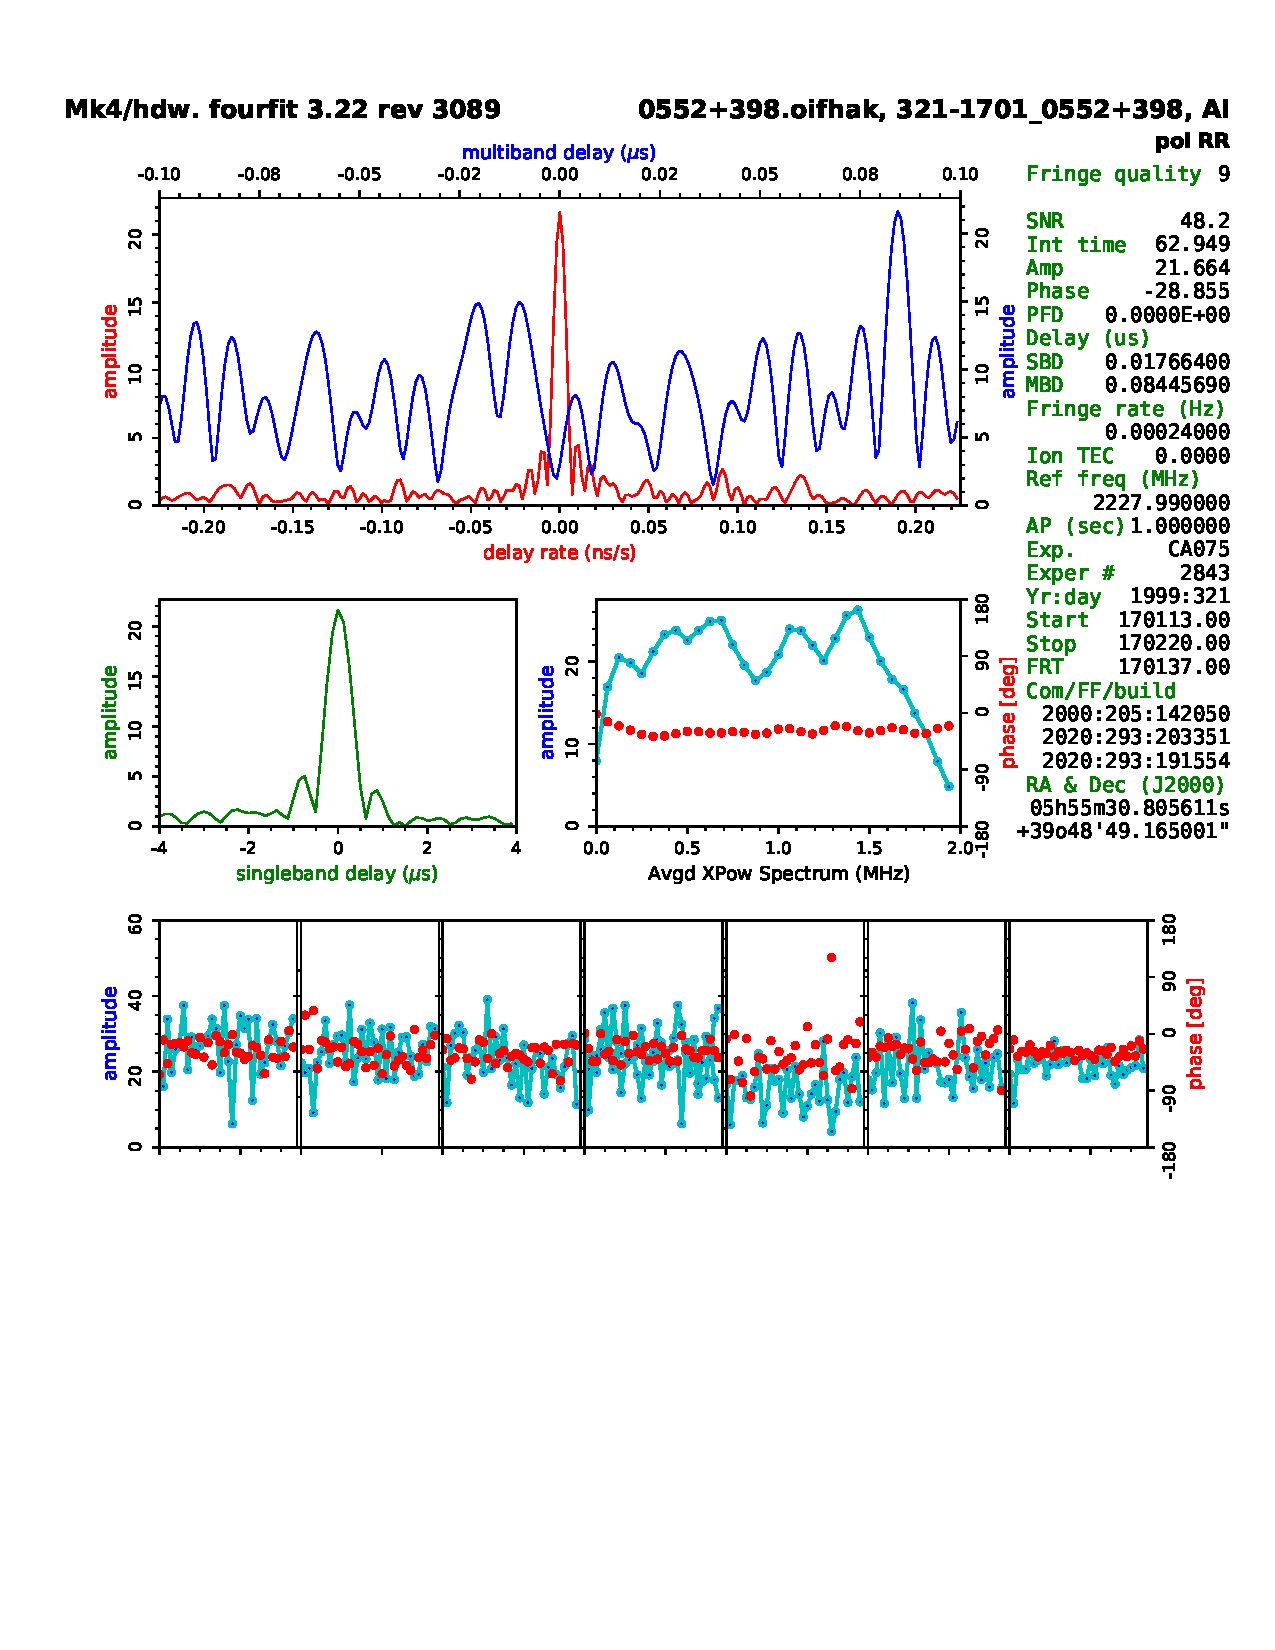
\includegraphics[width=0.7\textwidth]{fig/matplotlib-fringe-plot.pdf}
    \caption{Example of a fringe plot with Matplotlib.}
    \label{fig:matplotlib-fringe-plot}
\end{center}
\end{figure}


The plotting functions of \nuHOPS will be expanded, and will include hooks for users to insert their own plotting functions, interactive plots for reformatting, and simple extensibility to add features.
